% COEN 6314 project - two-page data report (DeepPCB preparation).
% Compile: pdflatex data_report.tex  (figures are read from fig/)
\documentclass[10pt,conference]{IEEEtran}
\usepackage[T1]{fontenc}
\usepackage{graphicx}
\usepackage{booktabs}
\usepackage{array}
\usepackage{amsmath}
\usepackage[hidelinks]{hyperref}
\newcommand{\fn}[1]{\texttt{\detokenize{#1}}}
\setlength{\tabcolsep}{3.2pt}

\begin{document}
\title{PCB Defect Detection Under Image Misalignment:\\ Data Report}
\author{\IEEEauthorblockN{Basma Kurany (40374114)}
\IEEEauthorblockA{COEN 6314 -- Introduction to Machine Learning, Concordia University\\ b\_kurany@live.concordia.ca}}
\maketitle

\begin{abstract}
This report describes the data used to test whether a compact learned detector can separate genuine PCB defects
from misalignment artefacts. It covers the DeepPCB source, the grouped train/validation/test partition, a quality
audit of the raw pairs, the seeded misalignment protocol, and the checks applied to every prepared image and box.
All numbers are produced by the scripts and JSON reports in the project repository.
\end{abstract}

\section{Source dataset}
DeepPCB~\cite{tang2019} contains 1{,}500 pairs of $640\times640$ binarised images: a defect-free \emph{template}
(reference) and an \emph{inspected} image of the same PCB region, aligned by the authors with template matching.
Each pair has 1--15 axis-aligned boxes (mean 6.7, 10{,}013 in total) labelled with one of six classes
(Table~\ref{tab:counts}). Defects are small: median box size $35\times33$\,px (18--173\,px wide), about 0.3\,\% of
the image area. Classes are close to balanced (largest/smallest ratio 1.33). Most defects were added artificially by
the dataset authors, which limits claims about real production defects. The official lists keep 1{,}000
\emph{trainval} and 500 \emph{test} pairs from 11 source-board \emph{groups} (folder names); group is the only
board identifier available.

\begin{table}[t]
\centering\footnotesize
\caption{Pairs and boxes per split after the grouped partition.}
\label{tab:counts}
\begin{tabular}{@{}lrrrrrrrr@{}}
\toprule
Split & Pairs & Open & Short & M.bite & Spur & Copper & P.hole & Boxes\\
\midrule
Train & 800 & 1005 & 825 & 1032 & 888 & 778 & 810 & 5338\\
Val   & 200 &  278 & 203 &  347 & 254 & 232 & 221 & 1535\\
Test  & 500 &  659 & 478 &  586 & 483 & 464 & 470 & 3140\\
\midrule
Total & 1500 & 1942 & 1506 & 1965 & 1625 & 1474 & 1501 & 10013\\
\bottomrule
\end{tabular}
\end{table}

\section{Partition}
The official 1{,}000/500 split is kept. About 20\,\% of trainval is held out for validation \emph{before} any
augmentation, grouped by source board so that no board appears in both train and validation. Every subset of
trainval groups containing 17--23\,\% of the pairs was scored by the $L_1$ distance between its class proportions
and those of all trainval; the best is group \fn{00041} (200 pairs, $L_1=0.059$), giving
\textbf{800 train / 200 val / 500 test}. All shifted variants of a pair inherit the pair's split.

Because the official test list was kept, the proposal's rule ``same board, same partition'' cannot hold for test:
7 of the 11 test groups also occur in trainval (168 test pairs), including 21 from the validation group. The other
332 test pairs come from four groups never seen in trainval (\fn{12000}, \fn{12100}, \fn{12300}, \fn{90100}), so a
group-held-out validation set is a reasonable proxy for test.

\section{Data-quality audit}
\textbf{Format.} All 3{,}000 images are $640\times640$; 62 images in 57 pairs are stored as 3-channel JPEGs and
were converted to single-channel. No label file is empty, malformed or out of bounds.

\textbf{Near-duplicates.} A difference hash over all templates gave 337 candidate pairs, re-checked at pixel level
(best offset within $\pm8$\,px, Jaccard $\geq0.9$ on copper and background). 40 duplicates were confirmed, all
inside a single group, which supports group as the board unit. None crosses train/val; three test pairs
(\fn{50600065}, \fn{92000114}, \fn{92000118}) duplicate a train pair and are flagged so results can be reported
with and without them.

\textbf{Native misalignment.} DeepPCB is described as aligned, but an integer search ($\pm8$\,px) for the offset
that minimises template/inspected disagreement finds 123 pairs (8.2\,\%) where some offset cuts the XOR area by at
least $1.5\times$: 75 train, 8 val, 40 test, typically 2--3\,px and up to 8\,px (Fig.~\ref{fig:native}). Their
``aligned'' condition is therefore already shifted. The offsets are stored per pair, so curves can be reported on all
pairs and, as a sensitivity check, on the 1{,}377 clean pairs (460 in test). 17 templates are near-blank
($<2$\,\% copper or background).

\begin{figure*}[t]
\centering
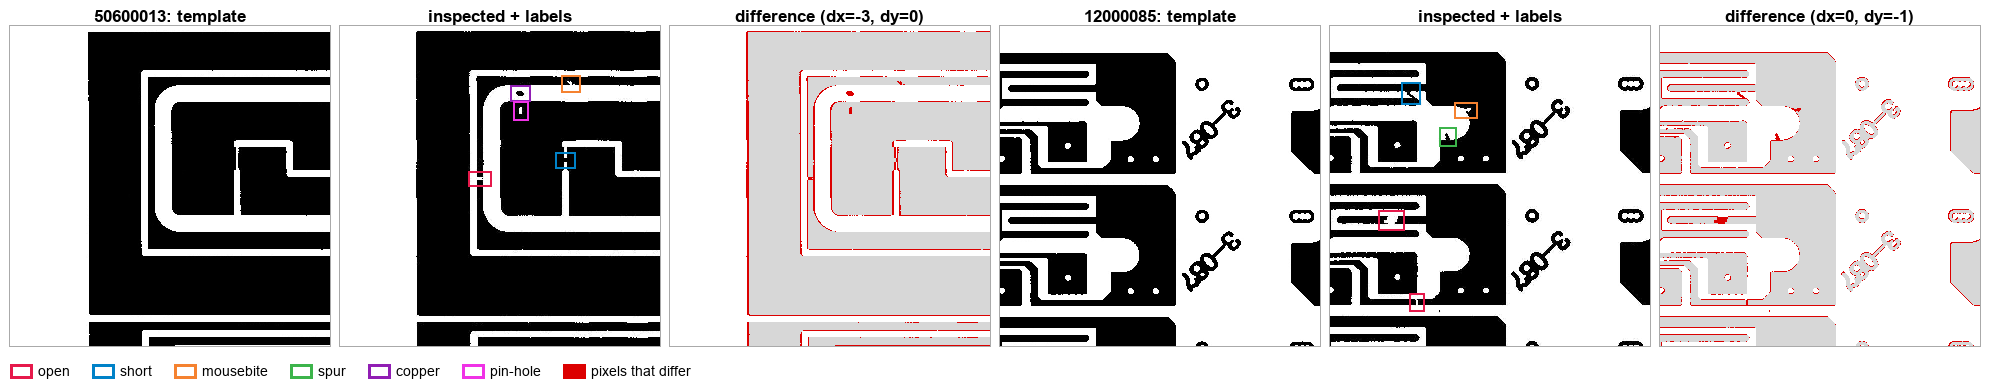
\includegraphics[width=\textwidth]{fig/native_misalignment_white_row.png}
\caption{Two pairs supplied as ``aligned'' but offset by 3\,px and 1\,px (offset found by the audit). Boxes show
the labelled defects by class; red marks pixels that differ between template and inspected image, outlining every
edge along the offset direction.}
\label{fig:native}
\end{figure*}

\section{Controlled misalignment protocol}
The reference is never modified; the inspected image and its boxes are moved together. For each validation and
test pair, ten conditions are generated (Table~\ref{tab:conds}): the pair as supplied (\fn{s0}); integer shifts of
1, 2, 3 and 5\,px along $x$ or $y$, each with a random sign; and a \emph{residual} condition $r$ with a sub-pixel
translation of 0.25--1.5\,px in a random direction plus a rotation in $[-0.5^\circ,0.5^\circ]$, which whole-pixel
registration cannot undo exactly. Integer shifts copy pixels (nearest-neighbour), so they add no interpolation
artefacts; $r$ uses bilinear interpolation, and rotated boxes are replaced by the axis-aligned envelope of their
four corners. Parameters are drawn from a generator seeded with $(6314,\text{pair ID})$, so both the baseline and
the detector read the \emph{same} files, independent of processing order. \textbf{Training
does see misalignment:} the non-augmented run uses the 800 pairs as supplied (75 already natively offset), and
the augmented run adds one random 1--5\,px shift and one residual copy of every pair (2,400 images, separate seed
stream; Section~VI).

\begin{table}[t]
\centering\footnotesize
\caption{Prepared inspected images (one reference per pair, 1{,}500 in total).}
\label{tab:conds}
\begin{tabular}{@{}lccccc@{}}
\toprule
Split & \fn{s0} & \fn{s1/2/3/5}$\times\{x,y\}$ & $r$ & Images & Boxes\\
\midrule
Train & 800 & -- & -- & 800 & 5{,}338\\
Val   & 200 & $8\times200$ & 200 & 2{,}000 & 15{,}350\\
Test  & 500 & $8\times500$ & 500 & 5{,}000 & 31{,}400\\
\bottomrule
\end{tabular}
\end{table}

\textbf{Borders and truncated defects.} Pixels uncovered by a shift are filled by edge replication. They lie inside
an 8\,px border (larger than the 5\,px shift and the $\approx$4\,px worst-case residual displacement) that is
excluded at evaluation: predictions centred there are discarded. A box whose \emph{original} position is within
14\,px of an edge ($8+6$ px maximum displacement) is marked \emph{ignore} in every condition, so the same defects
are treated as ``don't care'' at every shift: 258 boxes (2.6\,\%). Ignored boxes count as neither hit nor miss,
and a prediction matching one is not a false positive.

\section{Verification}
Two sets of checks were run: the pipeline's own QA scripts, and an independent audit written separately for this
report that re-decodes the raw DeepPCB files with a different library (Pillow/SciPy instead of OpenCV) and does not
reuse the pipeline code (Table~\ref{tab:qa}). The only difference found is one colour JPEG (\fn{44000020}), where the
two decoders' grey conversions differ on 2\,\% of pixels; its shifted copies still match its own \fn{s0} exactly.
Visual check sheets were also inspected for every condition (Fig.~\ref{fig:qa}).

\begin{table}[t]
\centering\footnotesize
\caption{Automated checks on the prepared data.}
\label{tab:qa}
\begin{tabular}{@{}p{0.72\linewidth}r@{}}
\toprule
Check & Result\\
\midrule
Pair lists, splits and \fn{boxes.csv} match raw files & 1500/1500\\
Reference images identical to raw templates & 1500/1500\\
\fn{s0} identical to raw inspected image (independent decoder) & 1499/1500\\
Integer-shift image $=$ \fn{s0} shifted by $(dx,dy)$, pixel-exact & 5600/5600\\
Box count, class, $(dx,dy)$ offset and ignore flag correct & 52088/52088\\
Non-ignored boxes inside valid region $[8,632]^2$ & 41220/41220\\
Residual images reproduced from stored parameters$^{\dagger}$ & 700/700\\
COCO files consistent with master CSV & 21/21\\
YOLO images with matching labels; zip CRC intact & 10200/10200\\
\bottomrule
\multicolumn{2}{@{}p{0.97\linewidth}@{}}{\scriptsize $^{\dagger}$Mean absolute difference $\leq0.22$ grey
levels in the valid region; ECC re-registration of 120 samples gives a maximum corner error of 0.05\,px.}
\end{tabular}
\end{table}

\begin{figure}[t]
\centering
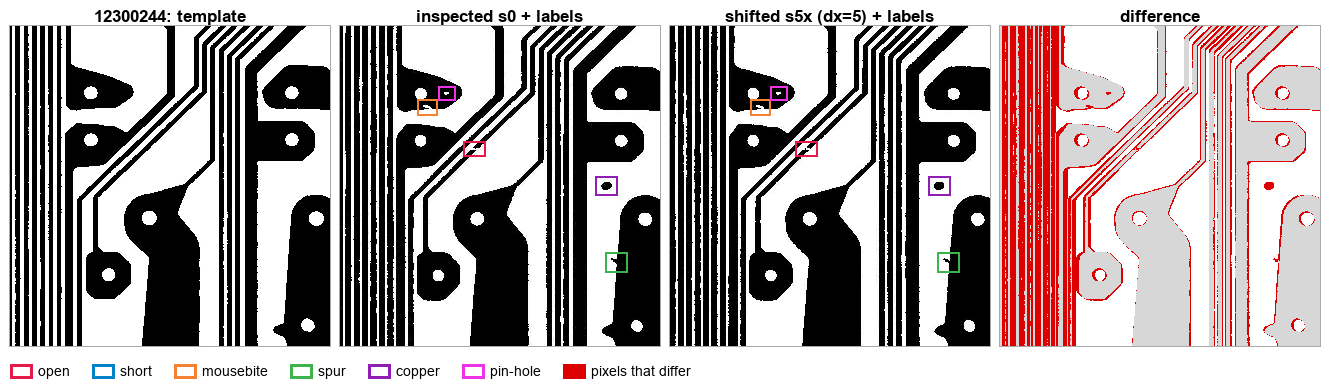
\includegraphics[width=\linewidth]{fig/check_s5x_white_row.png}
\caption{Label check for the 5\,px shift. Columns: template; inspected \fn{s0} with labels; shifted image with
shifted labels (boxes stay on their defects); difference in red, where the shift turns every track edge into a
false difference.}
\label{fig:qa}
\end{figure}

\section{Model-ready formats and reproducibility}
The master format is CSV: \fn{splits.csv} (pair, group, split, native offset, duplicate flag),
\fn{images.csv} (one row per inspected image with $dx$, $dy$, rotation) and \fn{labels.csv} (one row per box with
class and ignore flag). The same data are exported as 21 COCO files (ignore $\rightarrow$ \fn{iscrowd}) and as a
YOLO package in which each pair is one 3-channel image (reference, inspected, $|$difference$|$), so an
RGB-pretrained YOLOv10-Nano can be used unchanged. The augmented run (3$\times$ the images) trains for one
third of the epochs, so both runs take the same number of steps. Colour augmentation stays off, since it would
corrupt the difference channel; YOLO cannot encode ignore boxes, so evaluation reads \fn{labels.csv}. Everything
is rebuilt from the untouched DeepPCB download with \fn{scripts/run_all.sh}.

\section{Limitations}
Most defects are synthetic; validation is a single board group; each pair has only one residual variant; 123 pairs
are natively misaligned; and 168 test pairs share a board with trainval. These are reported alongside every
result rather than corrected.

\begin{thebibliography}{1}
\bibitem{tang2019} S.~Tang, F.~He, X.-L.~Huang, and J.~Yang, ``Online PCB defect detector on a new PCB defect
dataset,'' \emph{arXiv:1902.06197}, 2019.
\end{thebibliography}
\end{document}
